\section{R\&D-Agent}

\begin{figure*}[htbp]
\centering
  % \includegraphics[width=\linewidth]{Figures/Frame.pdf}
  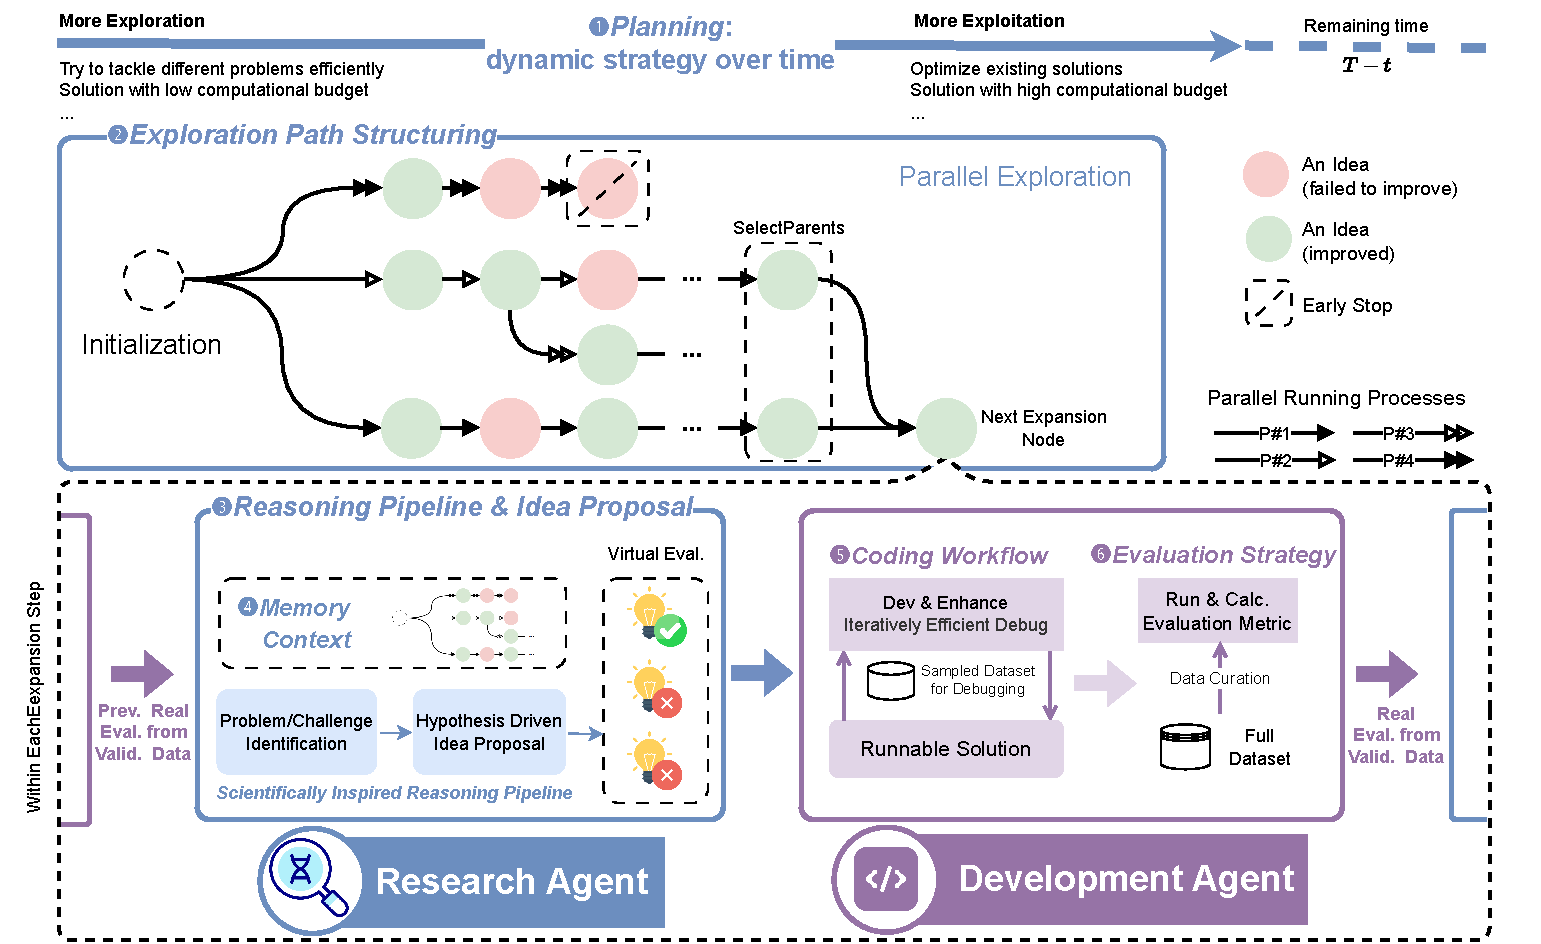
\includegraphics[width=\linewidth]{Figures/RD-Agent-FrameV02.pdf}
  \caption{Framework of R\&D-Agent. R\&D-Agent works in an iterative loop in which the Research Agent proposes ideas and the Development Agent implements them into runnable solutions to obtain feedback from data. By decoupling high-level research from low-level implementation, the framework efficiently explores the solution space through parallel exploration paths and iterative refinement, progressively converging on optimal solutions.}
  \label{fig:framework}
\end{figure*}

% - Framework
%
The architecture of the R\&D-Agent framework, illustrated in Figure~\ref{fig:framework}, addresses the core challenge of efficiently exploring optimal solutions in MLE. Built on a modular design principle, it decomposes the entire pipeline into distinct, configurable components. The framework orchestrates two specialized agents: a Research Agent that explores ideas through parallel paths, and a Development Agent that implements and iteratively refines these proposals. 

This modularity transforms agent development from monolithic construction into compositional optimization, enabling systematic exploration of a vast configuration space. Guided by human expert workflows, we navigated this space to identify an optimal design that achieves state-of-the-art performance on MLE-Bench, validating both our modular approach and the effectiveness of human-inspired reasoning patterns.

\subsection{Framework Overview}

Inspired by the common workflow of data scientists, the R\&D-Agent framework defines six key, extensible components, organized into two main phases: the Research Phase and the Development Phase. We introduce the \uline{F}ramework \uline{C}oncept (FC) of each component in this section.

\paragraph{The Research Phase.} The research phase aims to discover and refine promising ideas before committing to costly implementation. It consists of four primary components:

\begin{enumerate}[leftmargin=4ex]
    \item[\ding{182}] \textbf{FC-Planning:} This component focuses on the high-level allocation of exploration effort over time. Since data science tasks are sequential decision problems involving iterative trial-and-error, an effective plan must dynamically adjust the timing, budget, and guidelines for idea exploration. It adapts priorities and resources as new information emerges, managing the crucial trade-off between exploration and exploitation.

    \item[\ding{183}] \textbf{FC-Exploration Path Structuring:} This component determines how the solutions are organized and the historical solutions to which they will be referred. Strategies range from greedy chain-based approaches~\citep{nam2025mle}, which offer fast convergence at the risk of local optima, to tree-based search methods~\citep{liu2025ml,kulibaba2025kompeteai}, which maintain greater diversity at a higher computational cost. Our framework supports hybrid and adaptive designs that can combine these strengths.

    \item[\ding{184}] \textbf{FC-Reasoning Pipeline:} This component defines how knowledge from the \textit{memory context} is transformed into concrete research ideas. This process may include dataset analysis, hypothesis formulation, benefit justification, trade-off assessment, and implementable solution sketches. A clear, structured reasoning pipeline improves the quality, novelty, and feasibility of ideas, while supporting systematic evaluation before moving to development.

    \item[\ding{185}] \textbf{FC-Memory Context:} This component manages how accumulated knowledge, such as historical solutions, evaluation results, and insights, is stored, retrieved, and reused to inform the \textit{reasoning pipeline}. Well-structured memory enables knowledge transfer between iterations, reduces redundant exploration, and stabilizes long-horizon reasoning.
\end{enumerate}

\paragraph{The Development Phase.} The development phase turns the most promising research ideas into fully bug-free and evaluated solutions. It is composed of two key components:

\begin{enumerate}[leftmargin=4ex]
    \item[\ding{186}] \textbf{FC-Coding Workflow:} This component covers the process from a conceptual idea to bug-free code. It emphasizes modular design, efficient iterative debugging, and early detection of runtime issues. Techniques like rapid prototyping on sampled data can significantly shorten the development cycle while preserving correctness.

    \item[\ding{187}] \textbf{FC-Evaluation Strategy:} This component ensures reliable and consistent assessment of solution performance. A strong evaluation strategy involves choosing stable metrics, adhering to fixed validation settings, and using aggregated evaluations to reduce noise. This mitigates overfitting risks, filters out spurious high scores from underfitting, and ensures that iterative improvements reflect genuine performance gains rather than evaluation artifacts.
\end{enumerate}

\subsection{Framework Formulation}

We formalize the R\&D-Agent framework with the high-level algorithm presented in Algorithm~\ref{alg:rd_agent_framework}. The algorithm iteratively builds an exploration graph $\mathcal{G}$, by executing a loop composed of a Research Phase and a Development Phase until the time budget $T$ is met. Each component in the algorithm corresponds to the design aspects detailed in our framework overview. We call the loop in Algorithm~\ref{alg:rd_agent_framework} containing a research and development phase as \textbf{R\&D loop}.

\begin{algorithm}[H]
\SetAlgoLined
\DontPrintSemicolon
\SetKwInOut{KwIn}{Input}
\SetKwInOut{KwOut}{Output}
\SetKwInOut{KwNotation}{Notation}

\KwNotation{$\mathcal{G}_t$: exploration graph; $\pi_t$: plan; $\mathcal{N}_t$: parent nodes; $c_t$: context; $i_t$: idea; $x_t$: code; $s_t$: score.}
\KwIn{ML task $\mathcal{T}$, total time budget $T$}
\KwOut{Final solution $x^*$}
\BlankLine

$\mathcal{G} \gets \emptyset$ \tcp*{Initialize exploration graph}

\While{$\text{elapsed\_time}() < T$}
{
 \BlankLine
 
  \tcp{Research Phase}
  $\pi \gets \mathcal{P}(\mathcal{G}, \text{elapsed\_time()}, T)$ \tcp*{Planning}
  $\mathcal{N} \gets \text{SelectParents}(\mathcal{G}, \pi)$ \tcp*{Exploration Path Structuring}
  $c \gets \mathcal{M}(\mathcal{G}, \pi)$ \tcp*{Memory Context}
  $i \gets \mathcal{R}(c, \mathcal{N}, \pi)$ \tcp*{Reasoning Pipeline}
  \BlankLine
  
  \tcp{Development Phase}
  $x \gets \text{Dev}(i, \mathcal{N})$ \tcp*{Coding Workflow}
  $s \gets \text{Eval}(x, \mathcal{T})$ \tcp*{Evaluation Strategy}
  \BlankLine
  
  $\mathcal{G} \gets \mathcal{G} \cup \{(\mathcal{N}, i, x, s)\}$ \tcp*{Update exploration graph}
}

$x^* \gets \text{Submit}(\mathcal{G})$ \tcp*{Select and submit final solution}

\caption{High-Level Algorithm of the R\&D-Agent Framework}
\label{alg:rd_agent_framework}
\end{algorithm}



\subsection{A Human-Expert-Inspired Agent Design}
\label{sec:method-design}
The R\&D-Agent framework enables the systematic discovery of novel agent architectures. Guided by the workflows of human experts, we identified a specific, highly efficient agent configuration that establishes a new state-of-the-art on MLE-Bench. This section details the design choices for each of the six components in this SOTA configuration, with its core ideas illustrated in Figure~\ref{fig:framework}. We introduce the \uline{M}odule \uline{D}esign (MD) of each component in this section.

\begin{enumerate}[leftmargin=4ex]
\item [\ding{182}] \textbf{MD-Planning.}
Like human experts in scientific exploration, we quickly identify promising directions in the early stages and move to more sophisticated solutions later. To achieve this, we use a \uline{dynamic} planning strategy that adjusts over time. In the early stage (e.g., the first hour), the agent is given a limited computational budget, which discourages the use of heavy techniques such as ensembles or cross-validation. As promising directions emerge, the budget gradually increases, enabling more costly yet effective methods (e.g., ensembles, cross-validation) in later stages (e.g., at 4h). The plan also steers idea generation: early stages encourage novelty, while later stages focus on refining high-performing solutions with proven techniques.

\item [\ding{183}] \textbf{MD-Exploration Path Structuring.} 
Like human experts, R\&D-Agent explores multiple research directions in parallel and merges their strengths at the last stage for optimal solutions. We adopt an \uline{adaptive} DAG-based exploration structure guided by a core insight: initial implementations have disproportionate impact on exploration diversity, as subsequent steps are inherently path-dependent. Therefore, we maximize diversity in the first layer to establish distinct research directions, then greedily exploit the best solution within each branch while pruning sub-optimal paths. This design achieves efficient parallel exploration and result fusion.

\item [\ding{184}] \textbf{MD-Scientific Reasoning Pipeline.} Human data scientists typically follow a rigorous reasoning process to propose research ideas, which is a valuable distillation of human intelligence. Inspired by this, we propose a \uline{scientific multi-step} reasoning pipeline that begins by analyzing the current solution and dataset characteristics to identify the most critical problem (e.g., for a time-series dataset, mining temporal patterns is crucial for high performance). Rather than generating shallow ideas, the agent dives deeper into the problem, formulating hypotheses on why a proposed method would address it (e.g., an RNN can capture temporal dependencies in time-series data), and finally outputs an idea implementable by an LLM (e.g., training an LSTM\cite{graves2012long} to model dependencies). Since verifying ideas is more costly than generating them, we introduce a virtual evaluation strategy: the agent generates multiple ideas during reasoning, uses LLM-based assessments to select the most promising one, and sends only that to the development phase.

\item [\ding{185}] \textbf{MD-Memory Context.} 
We enhance \uline{collaborative} memory to enable knowledge sharing across parallel branches without sacrificing diversity. Each branch begins with a distinct idea and explores independently. After hypothesis generation, we augment each branch's context with two sources: the best ideas across all branches and a probabilistically sampled subset from others. The sampling kernel favors ideas that are topically similar and have higher scores, with more recent ideas weighted higher. An LLM then selects the most promising candidates from this enriched pool, accelerating convergence while maintaining exploration diversity.

\item [\ding{186}] \textbf{MD-Coding Workflow.} To improve efficiency, particularly for solutions with long runtimes, we adopt an \uline{efficient} and \uline{iterative debug} workflow. Our LLM-powered agent first samples a small, representative subset of the training data and enters a rapid prototyping loop: implementing the proposed idea, testing on this subset, and refining based on immediate feedback. This cycle continues until achieving a runnable and logically sound solution on the subset. Only validated solutions proceed to full-scale evaluation. This approach mirrors human rapid prototyping practices, significantly reducing development time by catching errors early and ensuring that computational resources are not wasted on flawed implementations. The workflow enables the agent to explore substantially more solution candidates within the same time budget.


\item [\ding{187}] \textbf{MD-Evaluation Strategy.} To ensure robust and reliable performance assessment, we implement an \uline{aggregated} evaluation strategy with standardized protocols. A key challenge in many MLE tasks is that evaluation logic is part of the agent's solution, causing inconsistent metrics and data splits that prevent fair comparison. We address this through two mechanisms. First, we enforce standardized data splitting: preparing fixed train-validation-test splits at the beginning of agent runs, with test data remaining entirely inaccessible for final grading. Second, beyond standard validation-based selection, we introduce an additional evaluation layer that collects top solutions from different exploration branches and evaluates them using consistent metrics on the same validation set. This aggregated approach ensures fair comparison across diverse solution strategies and enables more reliable selection of the best-performing solution for final submission.
\end{enumerate}

% \paragraph{\ding{187}Evaluation Strategy.} For robust performance assessment, we use a \uline{multiple} evaluation strategy.
% Unlike prior works in which the evaluation process changed along with the solution (the MLE task requiring the agent to also implement the evaluation), which could lead to inconsistencies, we use multiple metrics and keep the evaluation method fixed across different solutions to ensure more reliable results. \todo{it is hard to understand}
% We reserve part of the dataset to evaluate top solutions from different branches, which yields consistent comparisons and supports more accurate and efficient decision-making, even at a slight additional time cost.



% \subsection{Dedicated R\&D Role}
% Assigning dedicated R\&D roles helps tackle complex problems across a range of tasks, including machine learning engineering.
% When it comes to LLM-based MLE agents, the same design principles apply.
%   This approach mirrors how a team generally assigns different roles to people, such as researchers and developers, allowing us to use established research and development experience. In turn, the system can gather knowledge and insights from its practice, which match human intuition and experience, and can even inspire domain experts. These lessons can then be applied to new tasks.
%   On the other hand, there are various LLM foundation models with different strengths. For example, models like o1 are very good at reasoning and coming up with creative ideas, while models like GPT-4.1 are excellent at following instructions and implementing solutions. By assigning each agent the model that best fits its role, we can build a more effective team and achieve better results.
%
% % Concerete Design
% % - Research 
% % - Develop
%
% The research agent focuses on \textbf{learning} from experience and \textbf{exploration} of ideas. It proposes research directions to the development agent, analyzes the feedback it receives, and then refines its ideas. Through this cycle of learning and exploration, the research agent continuously improves and discovers better solutions.
%   The learning process relies on past or external experience. As new knowledge is gained, it is collected and organized into a knowledge base. This knowledge base helps the system refine its ideas or come up with new ones.
%   For exploration process and search strategies, we propose a novel multi-trace idea explorations, which enable parallel, diverse, and collaborative exploration of the solution space.
%   This part will be elaborated in section \ref{sec:multi-trace}.
%
%   The development agent focuses on \textbf{developing} and \textbf{enhancing} the engineering aspects of the proposed idea. The proposed idea usually only covers the key thoughts of the solution and is expressed in natural language as a high-level description that needs to be implemented.
%   In many cases, important engineering considerations are not fully addressed (e.g., the solution must finish running within a given resource budget); the development agent develops and enhances these aspects to ensure a more complete and practical solution.
%   To improve development efficiency, the process is divided into two phases: 1) developing a runnable solution and 2) running the solution. In the first phase, the development agent creates a runnable solution by iteratively debugging on a sampled dataset, similar to how human developers work. In the second phase, the development agent runs the solution on the full dataset to evaluate its performance.
%   In data science, training models usually involves large datasets. By having the development agent iterate on a smaller, sampled dataset first, the process becomes much faster and more efficient. This approach allows the agent to quickly test and refine solutions before running them on the full dataset, greatly speeding up overall development.



% \subsection{Multi-Trace idea explorations}
% \label{sec:multi-trace}
%
% In complex data science and machine learning engineering tasks, a single linear exploration path is often insufficient for discovering high-quality solutions. R\&D-Agent introduces a multi-trace exploration mechanism, which enables parallel, diverse, and collaborative exploration of the solution space. This section elaborates on the motivation behind this design and the architectural principles that underpin it.
%
% \textbf{Motivation and Design Principles:} One of the fundamental challenges in automated machine learning engineering is the risk of converging on suboptimal solutions due to the limitations of a single configuration. An exploration trace is inherently constrained by its initialization — including the choice of backend LLM, prompt structure, available tools, and supporting knowledge base. These constraints can heavily bias the exploration path, leading to stagnation or premature convergence. To address this, R\&D-Agent supports the parallel execution of multiple exploration traces, each configured with heterogeneous parameters. These include variations in prompt strategies, model backends, domain-specific tools, exploration heuristics, and even knowledge scopes. This diversity increases the likelihood of uncovering valuable insights from different perspectives and avoids the narrow search trajectories imposed by uniform assumptions.
%
% Beyond diversity, R\&D-Agent is built to scale. Its multi-trace system enables both logical and physical parallelism. Each trace operates as an independent research agent, executing asynchronously across compute nodes, containers, or threads. This design allows the system to scale horizontally across distributed environments, maximizing resource utilization and dramatically reducing time-to-solution. Such parallelism is especially important in high-complexity tasks where brute-force or single-threaded search would be computationally prohibitive.
%
% What's more, parallelism alone is not sufficient. Without coordination, multiple traces can waste resources on redundant explorations or persist with unpromising directions. To solve this, R\&D-Agent introduces cross-trace collaboration settings that govern how traces interact, evaluate progress, and make adaptive decisions. Each trace maintains a performance profile based on metrics such as solution quality, novelty, resource cost, and error resilience. A centralized module will track these profiles and makes dynamic decisions, such as terminating unproductive traces, spawning new ones with modified configurations, or initiating trace fusion. Importantly, traces are also able to share intermediate results — such as effective feature sets or partial models — creating a collective learning process where one trace’s success informs others.
%
% This principled combination of diversity, scalability, and collaboration forms the foundation of R\&D-Agent’s multi-trace exploration, driving efficient and robust progress in data-centric R\&D.


% \textbf{Multi-Trace Fusion for Stronger Solutions:}
% An essential outcome of multi-trace exploration is the ability to combine the strengths of multiple traces into a single, high-performing solution — a process we refer to as Multi-Trace Merge. Rather than selecting the best trace in isolation, R\&D-Agent provides a mechanism for compositional integration of partial results from several promising traces. This strategy allows the system to capitalize on the complementary advantages discovered by each trace.
%
% The fusion process operates at multiple granularities within the data science workflow. For instance, feature generation techniques from one trace may be combined with model architectures from another, and post-processing heuristics from a third. Each trace's components are evaluated and scored based on utility, novelty, compatibility, and performance impact. A configurable fusion strategy — such as greedy selection, weighted voting, or optimization-guided fusion — is then used to assemble the final solution.
%
% One of R\&D-Agent’s key strengths is its flexible and customizable fusion design. Users can define domain-specific control and fusion rules at each stage of the process:\begin{itemize}
%     \item During \textbf{trace evolution}, users can specify constraints for early stoping and spawning new traces based on performance thresholds, time used, or exploratory steps. 
%     \item During \textbf{ information exchange}, users can determine which intermediate outputs (e.g., code fragments, error logs, metrics) are shared across traces.
%     \item During the \textbf{fusion phase}, users can customize component compatibility rules, aggregation functions, or even plug in learned scoring models.
% \end{itemize}
%
% This flexibility ensures that R\&D-Agent can adapt to a wide range of application domains and engineering preferences. Whether in finance, healthcare, or industrial AI, the system’s composability and extensibility allow practitioners to shape exploration according to domain-specific requirements.
%
% By supporting modular integration and cross-trace learning, the Multi-Trace Merge mechanism not only improves the final solution quality but also accelerates convergence and strengthens the agent’s adaptability. This design is crucial in moving from isolated, trial-and-error automation toward intelligent, collective R\&D exploration.






% \begin{align*}
% & \mathcal{T} = \{1, 2, \dots, T\} \text{ is the set of traces,} \\[1mm]
% & \mathcal{H}^{(t)} = \{ (h_1^{(t)}, s_1^{(t)}), (h_2^{(t)}, s_2^{(t)}), \dots, (h_{m_t}^{(t)}, s_{m_t}^{(t)}) \}, 
%    \quad t \in \mathcal{T}, \\[1mm]
% & \mathcal{H} = \bigcup_{t \in \mathcal{T}} \mathcal{H}^{(t)} \text{ is the set of all historical hypotheses across traces,} \\[1mm]
% & (h^{\star},s^{\star}) = \argmax_{(h, s) \in \mathcal{H}} \text{LLM-score}(h,s) \quad \text{(globally best hypothesis selected by the LLM)}\\[1mm]
% & s_j^{\star} =\argmax_{(h^{(t)}, s^{(t)}) \in \mathcal{H}^{(t)}} (s^{(t)}) \quad \text{(best score in current trace)}
% \end{align*}

% \begin{align*}
% & \mathcal{M} = \{h_1^c, \dots, h_m^c\}, \quad 
% \mathcal{C} = \mathcal{H} \setminus \mathcal{H}^{(t)}, \quad 
% \mathbf{e}_i = \text{Embed}(h_i^c), \ \mathbf{h}_j = \text{Embed}(h_j),\\
% & S_{ij} = \cos(\mathbf{e}_i, \mathbf{h}_j) = \frac{\mathbf{e}_i \cdot \mathbf{h}_j}{\|\mathbf{e}_i\| \|\mathbf{h}_j\|}, 
% \quad h_i^c \in \mathcal{M}, \ h_j \in \mathcal{C}.\\
% & \Delta_{ij} = 
% \begin{cases}
% s_j^{\star} - s^{\star}, & \text{if higher is better} \\
% s^{\star} - s_j^{\star}, & \text{if lower is better}
% \end{cases},\\
% & \ell_{ij} = \alpha S_{ij} e^{-\gamma L} + \beta \tanh(\Delta_{ij}), \quad \ell_{ij} \in [-2, 2],\\
% & p_{ij} = \frac{\exp(\ell_{ij})}{\sum_{k} \exp(\ell_{ik})},\\
% & h^s  \sim \{p_{ij}\}
% \end{align*}







